\chapter{Introduction}
\label{ch:introduction}

\textbf{Foraging} is the process by which an organism searches for and exploits resources (typically food, but also mates, shelter, or other essential “targets”) when their locations are uncertain and sensory information is limited. When targets are sparse and the searcher has no map, the problem naturally becomes one of \textbf{random search}: how should a moving agent allocate effort between local exploration and long relocations to maximize encounter success. This question is not only ecological; it also underpins practical tasks such as environmental monitoring, inspection, and autonomous exploration in robotics~\cite{benichou2011intermittent}.

A major catalyst for the modern literature was the observation that some animal trajectories appear to mix many short moves with occasional long relocations, suggesting a \textbf{scale-free} search pattern~\cite{viswanathan1996albatross}. Early studies on wandering albatrosses popularized the idea that such movement can be captured by \textbf{Lévy search strategies}, i.e., random-walk models in which relocation lengths follow a heavy-tailed (power-law-like) distribution rather than having a characteristic scale~\cite{viswanathan1996albatross,shlesinger1986walks,shlesinger1993strange}. This motivated the \textbf{Lévy foraging hypothesis}, formulated in a minimal 2D setting with sparse targets and limited detection/memory, which argued that Lévy-like motion can be near-optimal under low information, and in particular highlighted inverse-square-type Lévy walks as a benchmark strategy for sparse search problems~\cite{viswanathan1999optimizing}. 

However, after more than two decades of work, the reported conclusions remain inconsistent: empirical re-analyses question the robustness of power-law fits~\cite{edwards2007revisiting,james2011assessing,plank2008optimal}, and theoretical results show that optimality can change when one modifies the objective, boundary conditions, bias, or the rules for revisiting targets~\cite{buldyrev2021comment,levernier2020inverse,palyulin2014levy,volpe2017topography}. This motivates a careful re-examination in which the search task is specified transparently and competing strategies are compared under identical assumptions.

\paragraph{Lévy-type relocations and scale-free trajectories.}
In this thesis the searcher moves at constant speed and executes \emph{relocations} whose lengths follow a heavy-tailed law. Concretely, the relocation length $L$ is sampled from a distribution with a power-law tail
\[
\Pr(L>\ell)\sim C\,\ell^{-\alpha}, \qquad 0<\alpha<2,
\]
where the tail exponent $\alpha$ controls the frequency of long relocations (smaller $\alpha$ corresponds to heavier tails). Because motion is realized at constant speed and simulated incrementally, the resulting process is strictly a \emph{L\'evy walk} (power-law relocations executed in continuous space at finite speed), rather than an idealized instantaneous-jump L\'evy flight.  Following common usage in the foraging literature~\cite{viswanathan1999optimizing,bartumeus2005animal}, we use the term ``L\'evy flight'' throughout the thesis as shorthand for this constant-speed, step-by-step process.  In sparse environments long relocations can reduce local oversampling, but whether this produces an interior optimum near $\alpha\approx 1$ depends on how detections are defined and on what performance criterion is optimized~\cite{bartumeus2002optimizing,raposo2003dynamical}.

The connection between Lévy statistics and fractal phenomena follows from the absence of a characteristic scale. Mandelbrot’s discussion of statistical self-similarity emphasizes how scale-free objects can look similar under magnification~\cite{mandelbrot1967coast}. Heavy-tailed relocations provide a dynamical instance of this idea: trajectories may exhibit similar visual structure across scales because no single relocation length dominates the motion.

\begin{figure}[t]
    \centering
    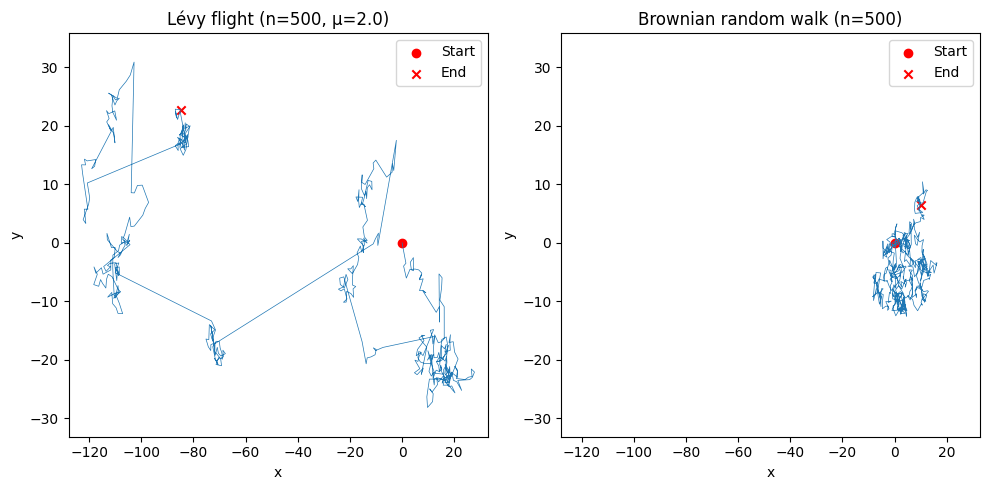
\includegraphics[width=0.9\linewidth]{images/levy_brownian.png}

    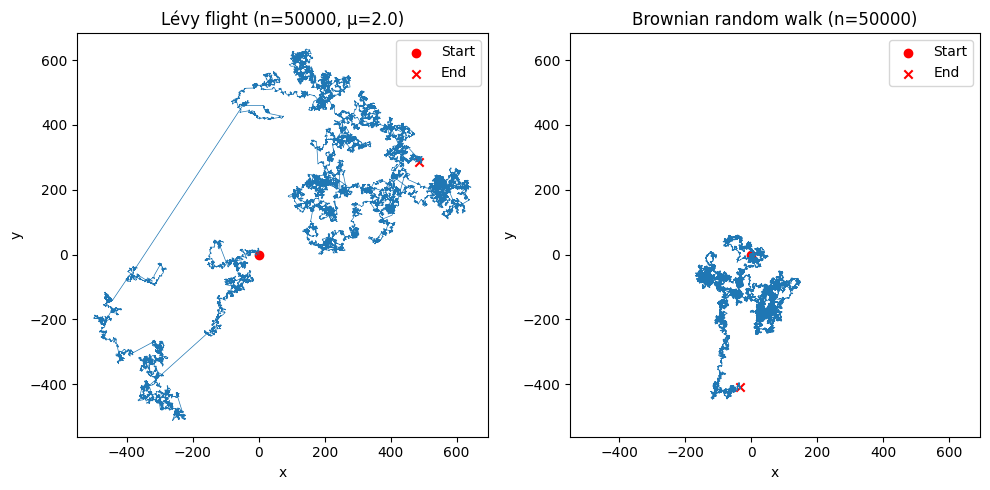
\includegraphics[width=0.9\linewidth]{images/levy_brownian1.png}
    \caption{Lévy-type (Cauchy) and Brownian trajectories of different lengths. Lévy-type paths combine many short steps with rare long relocations, while Brownian motion expands with a characteristic diffusion scale.}
    \label{fig:levy_brownian}
\end{figure}

Figure~\ref{fig:levy_brownian} contrasts a heavy-tailed trajectory and a Brownian one. Brownian motion produces strong local revisits and expands diffusively, whereas Lévy-type motion mixes local exploration with occasional long relocations. Importantly, this geometric intuition does not by itself determine optimality: in practice, the best exponent depends on (i) whether targets are depleted or revisitable, (ii) whether relocations are interrupted by detections, (iii) boundaries and finite-size effects, and (iv) whether one optimizes first-detection time or long-run encounter rate~\cite{buldyrev2021comment,levernier2020inverse,palyulin2014levy}.

\paragraph{Baseline model and why results disagree.}
A widely used baseline framework was proposed by Viswanathan \emph{et al.}~\cite{viswanathan1999optimizing}. Targets are randomly distributed in 2D; a searcher detects targets only within a finite radius $r_v$; if a target becomes visible the searcher moves to the nearest visible target; and if no target is visible the searcher chooses a random direction and a relocation length, then moves while continuously scanning within radius $r_v$. This formulation defines key parameters: detection range $r_v$, target density $\rho$, scan segment length $\Delta x$ used in simulation, finite horizon $T$ (or path budget), and the domain size and boundary conditions.

Two modeling points are especially consequential. First, the model distinguishes \emph{destructive} search (each target collected once) and \emph{nondestructive} search (targets can be revisited). In the nondestructive case, post-hit mechanics must be specified: common choices include a renewal time $\tau$ for targets or a forced departure (jump-off) distance $l_c$ from the hit target. These choices can shift, flatten, or eliminate an interior optimum in $\alpha$ and connect the model to revisitable-target and intermittent-search formulations~\cite{benichou2006twodimensional,benichou2011intermittent,lomholt2008levy,santos2004optimal}. Second, target representation in 2D is not innocuous: point targets are unrealistic because a continuous trajectory hits a point with probability zero; finite detection radius (and, effectively, finite target size) is required. Together with boundaries and discretization, such details help explain why different studies can reach contradictory conclusions, particularly when MFPT and throughput are not separated~\cite{james2011assessing,levernier2020inverse,plank2008optimal}.

\paragraph{Relevance.}
Because prior conclusions depend strongly on hidden modeling and implementation choices, a transparent and reproducible benchmark is needed to test Lévy-type optimality and to map which regimes favor which $\alpha$~\cite{edwards2007revisiting,james2011assessing,plank2008optimal}.

\paragraph{Main purpose of the research.}
The aim of this work is to construct a transparent and reproducible two-dimensional simulation benchmark for L\'evy walk search on infinite Poisson target fields, and to use this benchmark to determine---quantitatively and across a broad range of environmental and model parameters---under which conditions the inverse-square L\'evy exponent $\mu^* = 2$ is genuinely optimal, under which conditions the optimum shifts to ballistic or Brownian-like regimes, and how sensitively the optimal exponent depends on the post-detection strategy, target sparsity, and truncation parameters. Performance is evaluated using the pooled unique-capture rate and, for selected cases, the mean first-passage time (MFPT)~\cite{bartumeus2002optimizing,viswanathan1999optimizing}.

The specific research questions addressed are (stated in the
$\mu = \alpha + 1$ convention introduced in
Chapter~\ref{ch:methodology}):\phantomsection\label{sec:research_questions}
\begin{enumerate}
    \item \textbf{Existence and location of an optimum.}
    For which sparsity levels $\lambda/r_v$ and post-detection strategies does the efficiency curve $\lambda\eta(\mu)$ exhibit an interior maximum near $\mu \approx 2$ (equivalently $\alpha \approx 1$), and when does the optimum shift to the ballistic limit~\cite{buldyrev2021comment,levernier2020inverse}?
    \item \textbf{MFPT vs.\ throughput.}
    Does the exponent that minimizes MFPT coincide with the throughput-optimal exponent under identical settings~\cite{bartumeus2002optimizing,raposo2003dynamical}?
    \item \textbf{Sparsity dependence.}
    How does the optimal exponent $\mu^*$ change across two orders of magnitude in $\lambda/r_v$, and at what density does the L\'evy advantage disappear~\cite{bartumeus2005animal}?
    \item \textbf{Truncation sensitivity.}
    How do the truncation bounds $l_{\min}$ and $l_{\max}$ affect $\mu^*$ and the peak efficiency~\cite{chen2018tempered}?
    \item \textbf{Statistical convergence.}
    What number of flights and runs are required for stable estimates of $\mu^*$ and $\lambda\eta_{\max}$, particularly in the presence of trapping in non-destructive search~\cite{edwards2007revisiting,james2011assessing}?
\end{enumerate}

\paragraph{Scientific novelty.}
The novelty lies in a benchmarking methodology that makes conclusions about the optimal exponent comparable across assumptions: (i) four post-detection strategies (no-interrupt, teleport, Viswanathan destructive, Viswanathan non-destructive) are compared under identical target fields; (ii) MFPT and the pooled unique-capture rate are evaluated within the same framework; (iii) the optimal exponent $\mu^*$ (equivalently $\alpha^* = \mu^* - 1$) is mapped across two orders of magnitude in the sparsity ratio $\lambda/r_v$; and (iv) convergence studies and sensitivity analyses quantify the statistical reliability of the reported optima.

\paragraph{Statements for defense.}
\begin{enumerate}
    \item A reproducible 2D simulation framework for L\'evy walk search on an infinite Poisson target field with four post-detection strategies is implemented and validated~\cite{viswanathan1999optimizing}.
    \item The optimal L\'evy exponent converges to $\mu^* \approx 2$ ($\alpha^* \approx 1$) in the sparse-target limit for all four strategies (within the grid resolution $\Delta\mu = 0.1$), confirming the central prediction of the L\'evy foraging hypothesis.
    \item At high target density ($\lambda/r_v \leq 20$), the optimum shifts toward ballistic motion ($\mu^* = 1.0$--$1.4$) for strategies without trapping, demonstrating that L\'evy optimality is regime-dependent \cite{levernier2020inverse, bartumeus2005animal}.
    \item Non-destructive Viswanathan search exhibits pathological trapping at high density (revisit ratios $\sim 10^3$), creating spurious shifts of $\mu^*$ above~2 and necessitating pooled estimators with $R \geq 200$ runs.
\end{enumerate}

The remainder of the thesis is organized as follows.
Chapter~\ref{ch:literature_review} synthesizes evidence for and
against L\'evy-type optimality.
Chapter~\ref{ch:problem_statement} formalizes the problem and
notation.
Chapter~\ref{ch:methodology} describes the simulation methodology,
including the switch to the exponent $\mu = \alpha + 1$ used in
subsequent chapters.
Chapter~\ref{ch:experiments} presents numerical experiments:
phase diagrams of the optimal exponent, sensitivity and convergence
analyses, and comparison with analytical predictions.
Chapter~\ref{ch:discussion} summarizes results, states
conclusions, discusses limitations, and outlines possible
extensions.
